% !Mode:: "TeX:UTF-8"

\titlepage

\begin{frame}{说在前面}
	\linespread{1.5}
	  \begin{itemize}[<+-|alert@+>]
	    \item 如果对自己的作业成绩存在疑问,可以私信我查询本学期各次作业的成绩,
	    如果我的记录与实际情况不符,欢迎发难
	    \item 本子太烂了就换本新的吧
	    \item 本子还不算特别烂的下学期请继续使用
	    \item 新本子:贴照片,写上姓名、专业、学号、籍贯
	  \end{itemize}
\end{frame}

% \begin{frame}{需要注意的问题}
% 	\linespread{1.5}
% 	  \begin{itemize}%[<+-|alert@+>]
% 	    \item L'Hospital法则
% 	    \begin{itemize}
% 	      \item \it 只能应用于“$\df{\bm{0}}{\bm{0}}$”
% 	      和“$\df{\bm{\infty}}{\bm{\infty}}$”型
% 	      \item \it 及时使用无穷小代换进行简化
% 	      \item \it 不正规的符号:\b 
% 	      $\xlongequal{\footnotesize\mbox{“L”}}$、
% 	      $\xlongrightarrow{\footnotesize\mbox{“L'Hospital法则”}}$、
% 	      $\df{\bm{0}}{\bm{0}}$、$\df{\bm{\infty}}{\bm{\infty}}$
% 	    \end{itemize}
% 	    \item Taylor公式
% 	    \begin{itemize}
% 	      \item \it Taylor多项式不包含余项
% 	      \item \it 合并同次幂的系数
% 	      \item \it 尽量按照幂次由低到高排列,最后写余项
% 	    \end{itemize}
% 	  \end{itemize}
% \end{frame}

\begin{frame}{出现的问题}
	\linespread{1.5}
	  \begin{itemize}%[<+-|alert@+>]
	    \item 不画图!!!
	    \begin{itemize}
	      \item \b\it 不会画图
	      \item \b\it 不爱画图
	      \item \b\it 不想画图
	      \item \b\it 你懂的\ldots\ldots
	    \end{itemize}
	    \item 不交作业\ldots\ldots 不是问题:P
	  \end{itemize}
\end{frame}

\section{6.2 定积分的几何应用}

\begin{frame}
	\linespread{1.5}
	\ba{1. 设$S(t)$为直线$l_t:x+y=t(t\geq0)$下方位于正方形区域
	$D:0\leq x\leq 1,0\leq y\leq 1$内的\underline{面积},求$\dint_0^xS(t)\d t$。}
	\pause
	
% 	\bigskip
	
	\small 要点:\it
	$$S(t)=\left\{\begin{array}{ll}
		\df12t^2,& 0\leq t<1;\\ 1-\df12(2-t)^2, & 1\leq t <2;\\
		1,& t>2. 
	\end{array}\right.$$
	\ldots
	$$\dint_0^xS(t)\d t=\left\{\begin{array}{ll}
		\df16x^3,& 0\leq 0\leq x<1;\\ 
		\df16+(x-1)+\df16(2-x)^3, & 1<x\leq2;\\
		x-\df13,& x>2. 
	\end{array}\right.$$
\end{frame}

\begin{frame}
	\linespread{1.5}
	\ba{2.计算下列曲线的弧长:(1)$y=\ln(1-x^2)$,$0\leq x\leq\df12$}
	\pause
	
% 	\bigskip
	
	\small 解:\it
	弧长微元
	$$\alert{\d s=\sqrt{1+[y'(x)]^2}\d x}=\df{1+x^2}{1-x^2}\d
	x,\;(x\in\left[0,\df12\right]),$$
	故所求弧长
	$$s=\dint_0^{\frac12}\df{1+x^2}{1-x^2}\d x
	=\dint_0^{\frac12}\left[\df1{1+x}+\df1{1-x}-1\right]\d x
	=\ln3-\df12.$$
\end{frame}

\begin{frame}
	\linespread{1.5}
	\ba{2.计算下列曲线的弧长:
	(2)$\rho=a(1+\cos\theta)$,$0\leq\theta\leq2\pi$}
	\pause
	
% 	\bigskip
	
	\small 解:\it
	弧长微元
	$$\alert{\d s=\sqrt{\rho^2(\theta)+[\rho'(\theta)]^2}\d\theta}
	=2a\left|\cos\df{\theta}2\right|\d\theta,\;\theta\in[0,2\pi],$$
	故所求弧长
	$$s=\dint_0^{2\pi}2a\left|\cos\df{\theta}2\right|\d\theta
	=4a\dint_0^{\pi}\cos\df{\theta}2\d\theta
	=8a.$$
\end{frame}

\begin{frame}
	\linespread{1.5}
	\ba{3.设$D$是由曲线$y=\sin x+1$与三条直线$x=0,x=\pi,y=0$
	所围成的曲边梯形,求$D$绕$x$轴旋转一周所围成的旋转体的体积。
	}
	\pause
	
% 	\bigskip
	
	\begin{columns}
		\begin{column}{.5\textwidth}
			\begin{center}
				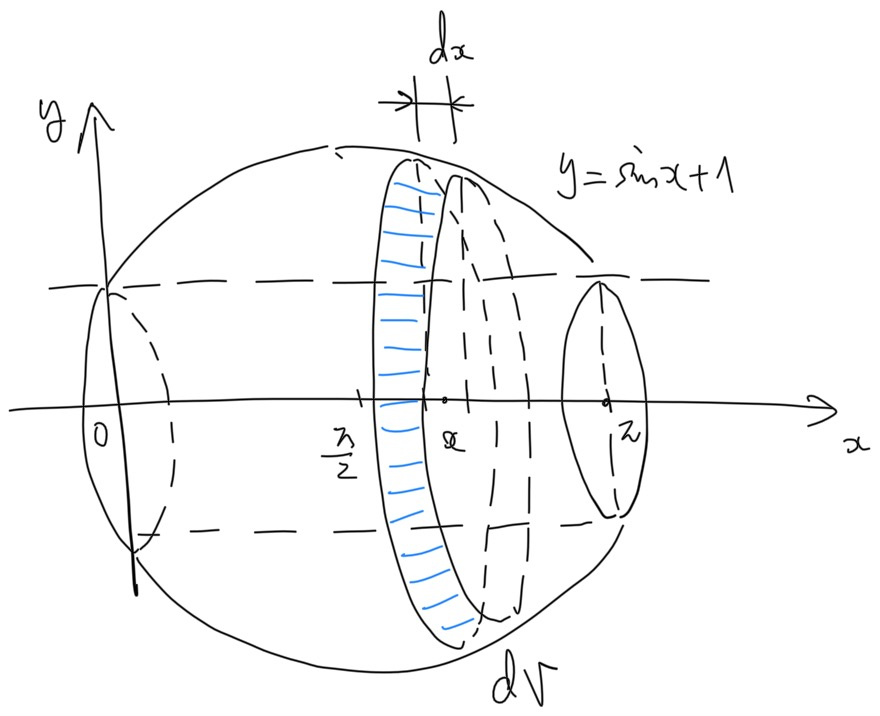
\includegraphics[width=.9\textwidth]{./images/ch6/sinx1cs.jpg}
		% 		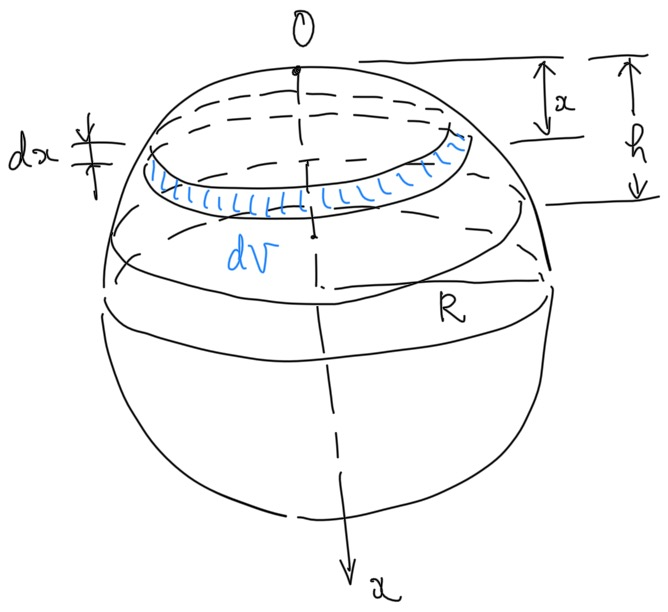
\includegraphics[width=6cm]{./images/ch6/topSp.jpg}
			\end{center}		
		\end{column}
		\begin{column}{.5\textwidth}
			\small 解:\it
			如图,体积微元$\d V=\pi y^2\d x$,	故所求体积
			$$
				V=\dint_0^{\pi}\pi(\sin x+1)^2\d x=\df32\pi^2.
			$$
		\end{column}
	\end{columns}
\end{frame}

\begin{frame}
	\linespread{1.5}
	\ba{4.证明球冠(球缺)的体积公式:$V=\pi h^2\left(R-\df{h}3\right)$,其中$R$为球
	的半径,$h<R$为球冠(球缺)的高。
	}
	\pause
	
% 	\bigskip
	
	\begin{columns}
		\begin{column}{.5\textwidth}
			\begin{center}
				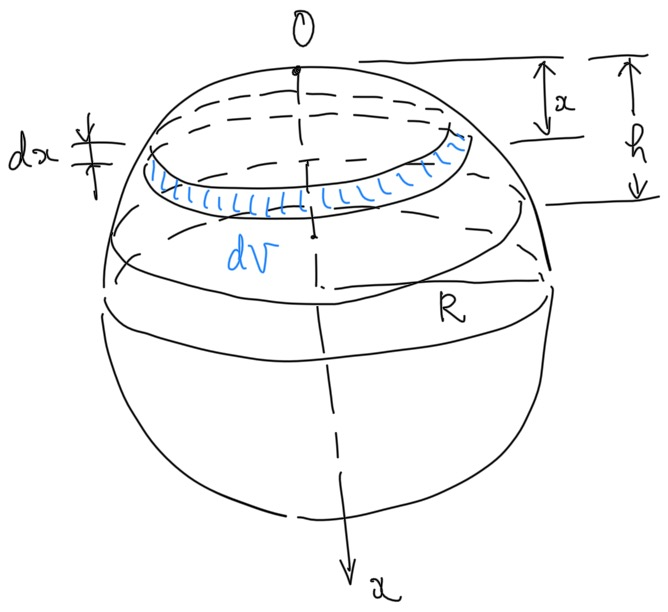
\includegraphics[width=.9\textwidth]{./images/ch6/topSp.jpg}
			\end{center}		
		\end{column}
		\begin{column}{.5\textwidth}
			\small 证:\it
			如图,体积微元
			$\d V=\pi[R^2-(R-x)^2]\d x=\pi(2Rx-x^2)\d x,$
			故球缺体积
			\begin{align*}
				V&=\dint_0^h\pi(2Rx-x^2)\d x\\
				&=\pi h^2\left(R-\df{h}3\right).
			\end{align*}
		\end{column}
	\end{columns}
\end{frame}

\begin{frame}
	\linespread{1.5}
	\ba{5.直线$y=x$将椭圆$x^2+3y^2=6y$分为两块,求两块的面积之比。
	}
	\pause
	
% 	\bigskip
	
	\begin{columns}
		\begin{column}{.45\textwidth}
			\begin{center}
				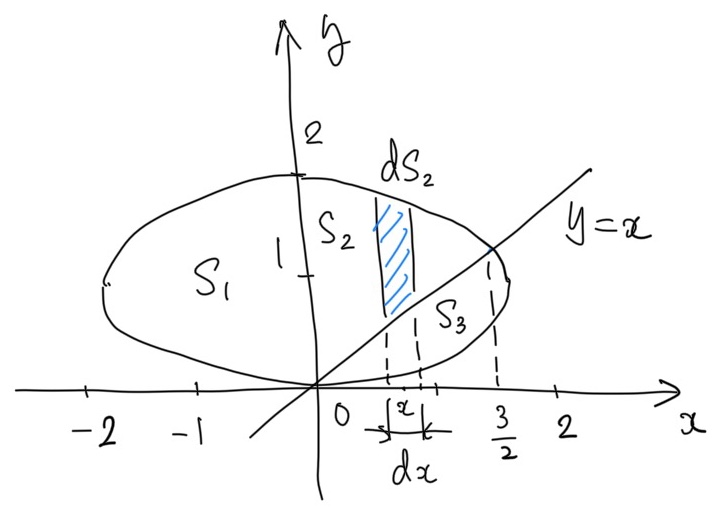
\includegraphics[width=.9\textwidth]{./images/ch6/ecXY.jpg}
			\end{center}		
		\end{column}
		\begin{column}{.55\textwidth}
			\small 要点:\it
			如图,
			\begin{align*}
				S_2&=\dint_0^{\frac32}\left(1+\sqrt{1-\df{x^2}3}-x\right)\d x\\
				&=\df34+\df{\sqrt3}6\pi.
			\end{align*}
			又$S_1=\sqrt3\pi$,故所求面积比为
			$$\df{S_1-S_2}{S_1+S_2}=\df{10\sqrt3\pi-9}
			{14\sqrt3\pi+9}$$
		\end{column}
	\end{columns}
\end{frame}

\begin{frame}
	\linespread{1.5}
	\ba{6.求曲线$y=\sqrt x$的一条切线,使之与该曲线及$x=0$、$x=2$
	共同所围面积最小。
	}
	\pause
	
% 	\bigskip
	
	\begin{columns}
		\begin{column}{.4\textwidth}
			\begin{center}
				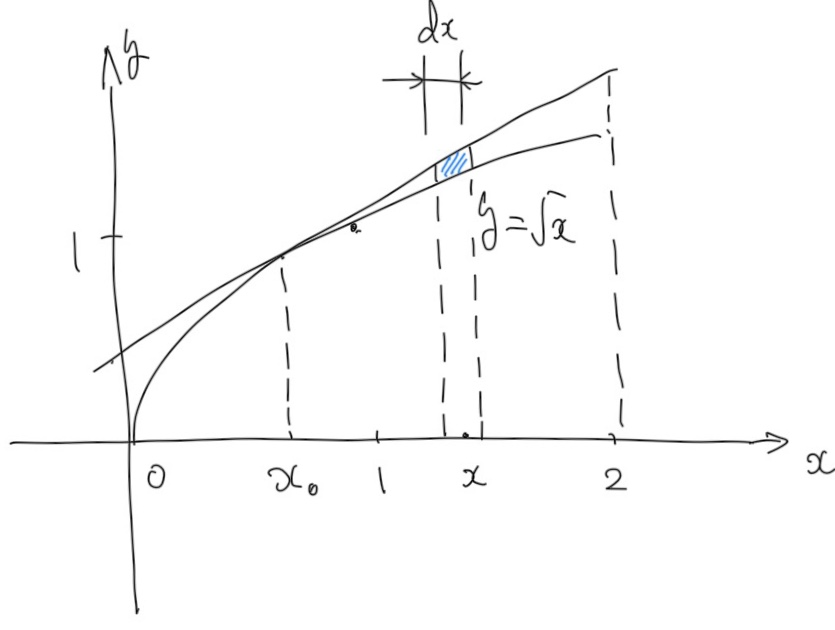
\includegraphics[width=\textwidth]{./images/ch6/ySqtXx.jpg}
			\end{center}		
		\end{column}
		\begin{column}{.6\textwidth}
			\small 解:\it
			如图,过曲线上一点$(x_0,\sqrt{x_0})$的切线为
			$y=\sqrt{x_0}+\df1{2\sqrt{x_0}}(x-x_0),$
			进而面积微元
			$\d S=\left[\df1{2\sqrt{x_0}}(x-x_0)+\sqrt{x_0}-\sqrt{x}\right]\d
			x$,$x\in[0,2]$。故所述面积
		\end{column}
	\end{columns}
	\small\it
	$$S=\dint_0^2\left[\df1{2\sqrt{x_0}}(x-x_0)+\sqrt{x_0}-\sqrt{x}\right]
	\d x=\df1{\sqrt{x_0}}+\sqrt{x_0}-\df{4\sqrt2}3.$$
	显然,当$x_0=1$时,该面积最小,此时对应切线为$y=\df12(x+1)$。
\end{frame}

\begin{frame}
	\linespread{1.5}
	\ba{8.求底面是半径为$R$的圆,而垂直于底面上一条固定直径的所有截面均为
	等边三角形的立体的体积。
	}
	\pause
	
	\bigskip
	
	\begin{columns}
		\begin{column}{.4\textwidth}
			\begin{center}
				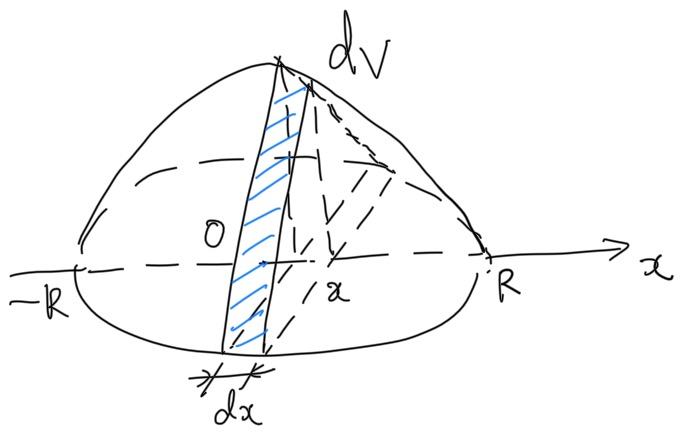
\includegraphics[width=\textwidth]{./images/ch6/rtSp.jpg}
			\end{center}		
		\end{column}
		\begin{column}{.6\textwidth}
			\small 解:\it
			如图,体积微元
			$$\d V=\sqrt3(R^2-x^2)\d x,\;x\in[-R,R],$$
			故所求体积
			$$V=\dint_{-R}^R\sqrt3(R^2-x^2)\d x=\df{4\sqrt3}3R^3.$$
		\end{column}
	\end{columns}
\end{frame}

\section{6.3 定积分的物理应用}

\begin{frame}
	\linespread{1.5}
	\ba{1.长度为$l$的细杆,均匀带电,总电量为$q\,(q<0)$,若在杆的延长线上,
	距离杆一端$x_0$处有一单位正电荷。现将单位正电荷从$x_0$处移动到无穷远,试求克服
	电场力所作的功。
	}
	\pause
	
	\begin{center}
		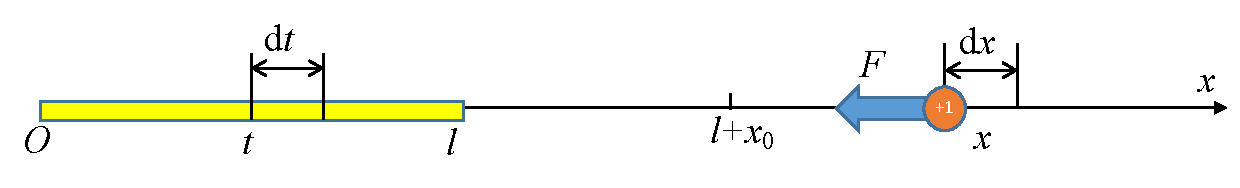
\includegraphics[width=.9\textwidth]{./images/ch6/eMove.pdf}
	\end{center}
	\small 解:\it
	如图,当单位正电荷位于$x(x>l)$处时,细杆上位置$t$处长度为$\d t$的一段对其产生的电场(吸引)力为
	$\d F=\df{kq\d t}{l(x-t)^2}$,$t\in[0,l]$
	故此时单位正电荷所受的总电场力为
	$$F=\dint_0^l\df{kq\d t}{l(x-t)^2}=\df{kq}l\left(\df1{x-l}-\df1x\right).$$
\end{frame}

\begin{frame}
	\linespread{1.5}
	\ba{1.长度为$l$的细杆,均匀带电,总电量为$q\,(q<0)$,若在杆的延长线上,
	距离杆一端$x_0$处有一单位正电荷。现将单位正电荷从$x_0$处移动到无穷远,试求克服
	电场力所作的功。
	}
	\pause
	
	\begin{center}
		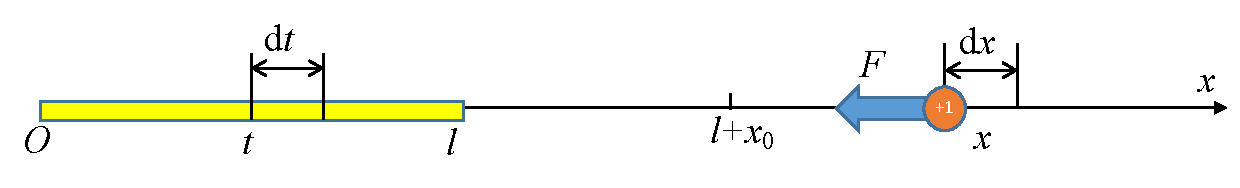
\includegraphics[width=.9\textwidth]{./images/ch6/eMove.pdf}
	\end{center}
	\small \it
	克服该力的作用,单位正电荷向远处移动$\d x$,需要做的功为
	$$\d W=F\d x=\df{kq}l\left(\df1{x-l}-\df1x\right)\d x,
	\quad x\in[l+x_0,+\infty)$$
	故所求克服电场力所需做的总功为
	$$W=\dint_{l+x_0}^{+\infty}\df{kq}l\left(\df1{x-l}-\df1x\right)\d x
	=\df{kq}l\ln\left(1+\df{l}{x_0}\right).$$
\end{frame}

\begin{frame}
	\linespread{2}
	\begin{columns}
		\begin{column}{.4\textwidth}
			\ba{2.星形线的参数方程为:$x=a\cos^3t,y=a\sin^3t$,设其上每一点处的密度
			等于其到原点距离的\underline{立方的}$k$倍,在原点处放置一单位质点,
			求星形线在第一象限的部分对该质点的引力。
			}	
		\end{column}
		\begin{column}{.6\textwidth}
			\begin{center}
				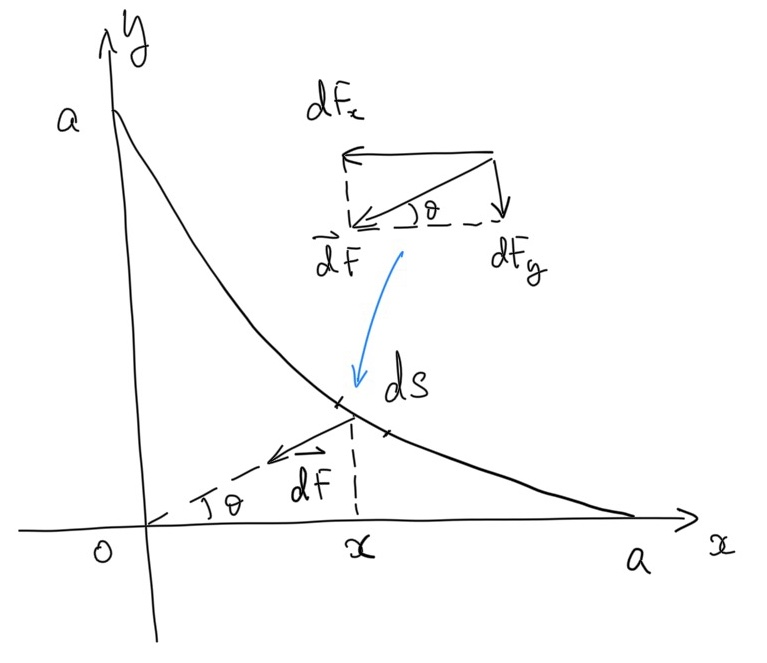
\includegraphics[width=.9\textwidth]{./images/ch6/starGr.jpg}
			\end{center}
		\end{column}
	\end{columns}
\end{frame}

\begin{frame}
	\linespread{1.5}
	\ba{3.边长为$a$和$b$的矩形薄板,与水面成角度$\theta$斜沉于水中,长边
	平行于水面,最低处深度为$h$,设$a<b$,水的密度$\rho=1$,求水对于薄板上侧
	的总压力。
	}
	\pause
	
	\bigskip
	
	\begin{columns}
		\begin{column}{.45\textwidth}
			\begin{center}
				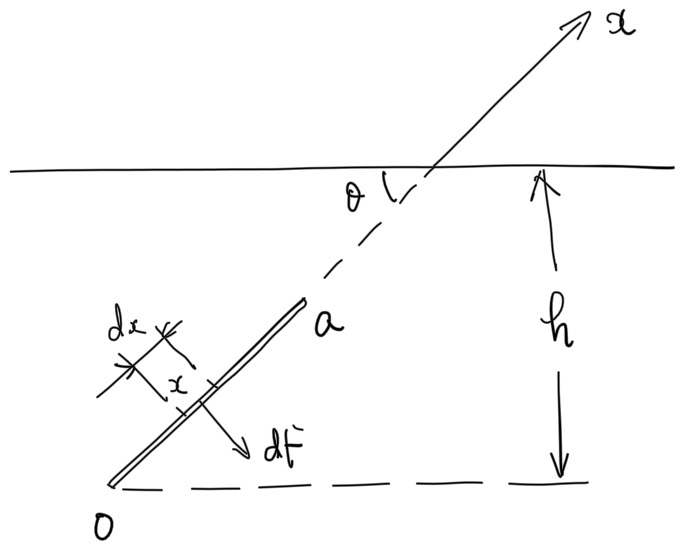
\includegraphics[width=\textwidth]{./images/ch6/waterPlane.jpg}
			\end{center}		
		\end{column}
		\begin{column}{.55\textwidth}
			\small 解:\it
			如图,压力微元
			$$\d F=g(h-x\sin\theta)b\d x,$$
			故所求压力
			\begin{align*}
				F&=\dint_0^ag(h-x\sin\theta)b\d x\\
				&=bg\left(ha-\df{a^2}2\sin\theta\right).
			\end{align*}
		\end{column}
	\end{columns}
\end{frame}

\begin{frame}
	\linespread{1.5}
	\ba{4.一个物体按照$x=t^3$作直线运动,已知其所受阻力等于其速度平方的$1.5$倍,
	求其从原点出发移动$1000$米时克服阻力所做的功。
	}
	\pause
	
	\begin{center}
		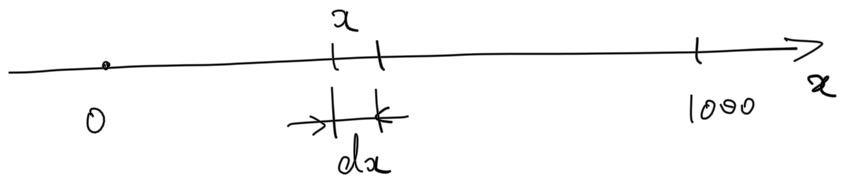
\includegraphics[width=.9\textwidth]{./images/ch6/moveSt.jpg}
	\end{center}
	\small 解:\it
	如图,功的微元$\d W=\df32(x'_t)^2\d x=\df{81}2t^6\d t$,故所求总功
	$$W=\dint_0^{10}\df{81}2t^6\d t=\df{81}{14}\times10^7.$$
\end{frame}

\begin{frame}
	\linespread{1.5}
	\ba{5.用铁锤将一铁钉击入木板,设木板对铁钉的阻力与铁钉已进入木板的深度成正比,
	已知第一次敲击后,铁钉进入木板$1$cm,假设每次敲击所做的功相同,问第二次敲击
	后,铁钉又将进入木板多少?
	}
	\pause
	
	\bigskip
	
	\begin{columns}
		\begin{column}{.35\textwidth}
			\begin{center}
				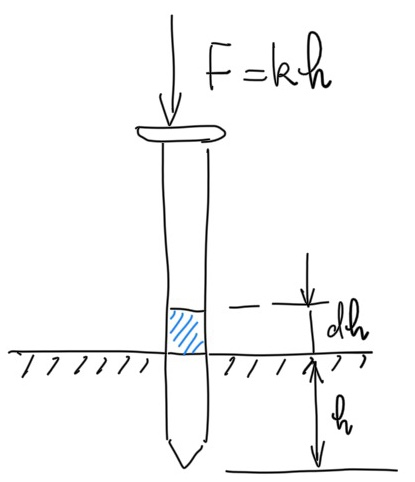
\includegraphics[width=\textwidth]{./images/ch6/nailSt.jpg}
			\end{center}		
		\end{column}
		\begin{column}{.65\textwidth}
			\small 解:\it
			如图,功的微元$\d W=kh\d h,$
			由已知第一次敲击时所做的功$W_1=\dint_0^1kh\d h=\df k2,$
			设第二次敲击后到达的深度为$h_2$,则与之相对应的功
			$$W_2=\dint_1^{h_2}kh\d h=\df k2(h^2_2-1)=W_1=\df k2,$$
			解得$h_2=\sqrt2$。故第二次敲击后,铁钉又将进入的深度为
			$\sqrt2-1$。
		\end{column}
	\end{columns}
\end{frame}

\begin{frame}
	\linespread{1.5}
	\ba{6.一个半径为$R$,圆心角为$\theta$的圆弧形细棒,其线密度为$\mu$,
	在圆心处放置一单位质点,问细棒对该质点的引力大小为多少?方向如何?
	}
	\pause
	
	\bigskip
	
	\begin{columns}
		\begin{column}{.4\textwidth}
			\begin{center}
				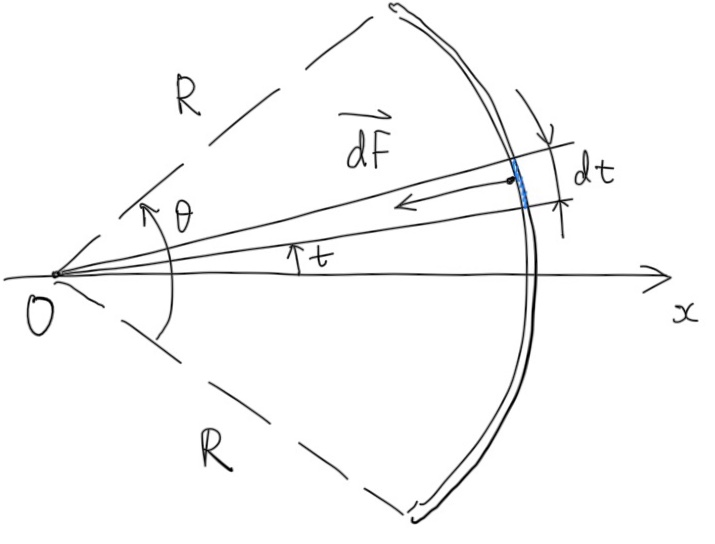
\includegraphics[width=\textwidth]{./images/ch6/theSphGr.jpg}
			\end{center}		
		\end{column}
		\begin{column}{.6\textwidth}
			\small 要点:\it
			引力微元
			$|\bm{\d F}|=\df{G\mu\d t}R,$,故
			\begin{align*}
				\d F_x&=|\bm{\d F}|\cos t=\df{G\mu\cos t\d t}R,\\
				\d F_y&=|\bm{\d F}|\sin t=\df{G\mu\sin t\d t}R,
			\end{align*}
			所求引力大小为$\df{2G\mu}{R}\sin\df{\theta}2$,沿$x$轴指向原点方向。
		\end{column}
	\end{columns}
\end{frame}